\documentclass[a4paper, 12pt]{article}
\usepackage[utf8x]{inputenc}
\usepackage{cmap}
\usepackage[english, russian]{babel}
\usepackage{indentfirst}
\usepackage[left=20mm, top=20mm, right=20mm, bottom=20mm]{geometry}
\usepackage{tikz}
\usepackage{float}
\usepackage{amsmath, amsfonts, amssymb}
\usepackage{graphicx}
\usepackage{fancybox, fancyhdr}
\usepackage{hyperref}
\usepackage{listings}
\usepackage{caption}
\usepackage{subcaption}
\usepackage{xcolor}
\pagestyle{fancy}
\fancyhf{}
\fancyhead[L]{Лабораторная работа №6}
\fancyhead[R]{Техническое зрение}
\fancyfoot[C]{\thepage}
\graphicspath{{images/}}
\usetikzlibrary{patterns}
\definecolor{LightGray}{gray}{0.95}
\definecolor{LightGray2}{gray}{0.7}
\lstdefinestyle{pycode}{
    language=Python,
    basicstyle=\footnotesize\ttfamily,
    numbers=left,
    numberstyle=\scriptsize\color{gray},
    stepnumber=1,
    numbersep=5pt,
    backgroundcolor=\color{LightGray},
    showspaces=false,
    showstringspaces=false,
    showtabs=false,
    tabsize=4,
    captionpos=b,
    breaklines=true,
    breakatwhitespace=false,
    frame=single,
    rulecolor=\color{LightGray2},
    linewidth=\linewidth,
    keywordstyle=\color{blue}\bfseries,
    commentstyle=\color{green!40!black},
    stringstyle=\color{purple},
    escapeinside={\%*}{*)},
    inputencoding=utf8x,
    xleftmargin=0pt,
    framexleftmargin=0pt,
    framexrightmargin=0pt
}
\lstset{style=pycode}
\hypersetup{
    colorlinks=true,
    linkcolor=blue,
    filecolor=magenta,
    urlcolor=cyan,
    pdftitle={contents setup},
    pdfpagemode=FullScreen,
}
\setlength{\parskip}{1.5mm}
\setlength{\headheight}{15pt}
\setlength{\footskip}{15pt}
\allowdisplaybreaks
\DeclareMathOperator{\sinc}{sinc}
\newcommand{\frc}[2]{\raisebox{2pt}{$#1$}\big/\raisebox{-3pt}{$#2$}}

\begin{document}
    \begin{titlepage}

        \begin{center}
        
\includegraphics[width=0.3\textwidth]{itmo.png} % requires itmo.png in /images folder
        \vfill

        Федеральное государственное автономное образовательное учреждение высшего образования
        «Национальный Исследовательский Университет ИТМО»\\

        \vfill
        {\large\bf ЛАБОРАТОРНАЯ РАБОТА №6}\\
        {\large\bf ПРЕДМЕТ «ТЕХНИЧЕСКОЕ ЗРЕНИЕ»}\\
        {\large\bf ТЕМА «МОРФОЛОГИЧЕСКИЙ АНАЛИЗ ИЗОБРАЖЕНИЙ»}
        \vfill

        \begin{flushright}
            \begin{minipage}{.45\textwidth}
            {
                \hbox{Преподаватель:}
                \hbox{Шаветов C. В.}
                \hbox{}
                \hbox{Выполнили:} 
                \hbox{Румянцев А. А.}
                \hbox{Чебаненко Д. А.}
                \hbox{Овчинников П. А.}
                \hbox{}
                \hbox{Поток: ТЕХ. ЗРЕНИЕ 2.1}
                \hbox{Факультет: СУиР}
                \hbox{Группа: R3241}
            }
            \end{minipage}
        \end{flushright}

        \vfill

        Санкт-Петербург\\
        2024
        \end{center}
    \end{titlepage}

    \tableofcontents

    \newpage
    \section{Цель работы}
    Освоение принципов математической морфологии в области обработки и анализа изображений.

    
    \section{Теоретические сведения}
    Математическая морфология в обработке изображений применяется для фильтрации шумов, сегментации
    объектов, выделения контуров, поиска заданного объекта на изображении, вычисления "скелета" образа и
    других преобразований. Далее рассмотрим базовые морфологические операции над изображением $A$ структурным
    элементом $B$.


    \section{Задание 1}
    Выберем произвольное изображение, содержащее дефекты формы (внутренние <<дырки>> или внешние <<выступы>> объектов).
    Пусть это будет мухомороподобный перченый флаг Японии, нарисованный в Paint. Так как фон изображения белого цвета,
    добавим рамку вокруг картинки для видимости границ.
    \begin{figure}[H]
        \centering
        \fbox{
\includegraphics[scale=0.365]{base_morf.png}}
        \captionsetup{skip=0pt}
        \caption{Изображение для задания 1}
        \label{fig:izt1}
    \end{figure}
    Далее будем пробовать различные морфологические операции для устранения черных точек, белых точек и красных выступов.


    \subsection{Дилатация}
    Дилатация (расширение, наращивание): $A\oplus B$, расширяет бинарный образ $A$ структурным элементом $B$. Данная операция
    увеличивает белые области на изображении. Применим ее к исходной картинке и посмотрим результат.
    \begin{figure}[H]
        \centering
        \fbox{
\includegraphics[scale=0.27]{dil_bm.png}}
        \captionsetup{skip=0pt}
        \caption{Применение дилатации к исходному изображению}
        \label{fig:dil1}
    \end{figure}
    Видим, что белые <<дырки>> внутри красного круга стали больше, черные меньше. Радиус окружности уменьшился, частично
    срезались выступы по краям.


    \subsection{Эрозия}
    Эрозия (сжатие, сужение): $A\ominus B$, сужает бинарный образ $A$ структурным элементом $B$. Эта операция уменьшает
    белые области на изображении. Применим ее к оригинальной картинке и сравним с ней результат.
    \begin{figure}[H]
        \centering
        \fbox{
\includegraphics[scale=0.27]{er_bm.png}}
        \captionsetup{skip=0pt}
        \caption{Применение эрозии к исходному изображению}
        \label{fig:er1}
    \end{figure}
    Можем заметить, что белые <<дырки>> внутри красного круга пропали, черные увеличились. Радиус круга и дефекты по его краям
    стали больше. Наблюдаем эффект, обратный дилатации. Результат зависит от количества итераций, то есть от того, сколько раз
    операция была применена к изображению. Если выбрать меньшее количество итераций в данном пункте, то белые <<дырки>> уменьшатся,
    но не пропадут. То же самое в пункте про дилатацию -- если сделать больше итераций, то черные <<дырки>> полностью исчезнут.


    \subsection{Открытие}
    Открытие (отмыкание, размыкание, раскрытие): $(A\ominus B)\oplus B$, удаляет внешние дефекты бинарного образа $A$ структруным
    элементом $B$. Состоит из последовательного применения эрозии и дилатации. Применим операцию к изначальному изображению.
    \begin{figure}[H]
        \centering
        \fbox{
\includegraphics[scale=0.27]{op_bm.png}}
        \captionsetup{skip=0pt}
        \caption{Применение открытия к исходному изображению}
        \label{fig:op1}
    \end{figure}
    Видим, что белые <<дырки>> пропали, черные остались нетронуты. Радиус красной окружности не изменился. В местах
    выступов круг начал сливаться с ними, что означает, что операция сгладила внешние дефекты.


    \subsection{Закрытие}
    Закрытие (замыкание): $(A\oplus B)\ominus B$, удаляет внутренние дефекты бинарного образа $A$ структурным элементом $B$.
    Состоит из последовательного применения дилатации и эрозии. Применим данную операцию к исходному изображению и посмотрим
    результат.
    \begin{figure}[H]
        \centering
        \fbox{
\includegraphics[scale=0.27]{cl_bm.png}}
        \captionsetup{skip=0pt}
        \caption{Применение закрытия к исходному изображению}
        \label{fig:cl1}
    \end{figure}
    Черные <<дырки>> внутри круга исчзели, белые почти не изменились. Внешние дефекты окружности немного срезались, но
    вместе с некоторыми ее частями.


    \subsection{Комбинации}
    Попробуем сначала применить 4 раза эрозию, потом 9 раз дилатацию. Также применим последовательно открытие и закрытие. Посмотрим на результат.
    \begin{figure}[H]
        \centering
        \fbox{
\includegraphics[scale=0.27]{er_then_dil_bm.png}}
        \captionsetup{skip=0pt}
        \caption{Применение эрозии и дилатации к исходному изображению}
        \label{fig:erdil1}
    \end{figure}
    \begin{figure}[H]
        \centering
        \fbox{
\includegraphics[scale=0.27]{op_then_cl_bm.png}}
        \captionsetup{skip=0pt}
        \caption{Применение открытия и закрытия к исходному изображению}
        \label{fig:opcl1}
    \end{figure}
    Как видим, оба варианта выглядят неплохо. Пропали внутренние дефекты, внешние только сглажены, так как убрать их
    полностью без потери большей части информации о рассматриваемом объекте (красном круге) не получается (радиус окружности
    становится либо сильно больше, либо сильно меньше оригинала).


    \subsection{Листинг для задания 1}
    Задание было выполнено на языке программирования Python с использованием библиотек numpy и opencv-python.
    \begin{lstlisting}[label=task1, caption=Программа для базовых морфологических операций]
    import cv2
    import numpy as np

    def dilate(I, ker_sz=(5, 5), iters=1):
        ker = np.ones(ker_sz, np.uint8)
        return cv2.dilate(I, ker, iterations=iters)
    
    def erode(I, ker_sz=(5, 5), iters=1):
        ker = np.ones(ker_sz, np.uint8)
        return cv2.erode(I, ker, iterations=iters)
    
    def opening(I, ker_sz=(5, 5)):
        ker = np.ones(ker_sz, np.uint8)
        return cv2.morphologyEx(I, cv2.MORPH_OPEN, ker)
    
    def closing(I, ker_sz=(5, 5)):
        ker = np.ones(ker_sz, np.uint8)
        return cv2.morphologyEx(I, cv2.MORPH_CLOSE, ker)

    if __name__ == '__main__':
        path = 'tv_lab6'
        src = 'source'
        render = 'renders'
        
        bm = cv2.imread(f'{path}/{src}/base_morf.png', cv2.IMREAD_COLOR)
    
        dil = dilate(bm, iters=3)
        er = erode(bm, iters=4)
        op = opening(bm, ker_sz=(15, 15))
        cl = closing(bm, ker_sz=(18, 18))
        cv2.imwrite(f"{path}/{render}/dil_bm.png", dil)
        cv2.imwrite(f"{path}/{render}/er_bm.png", er)
        cv2.imwrite(f"{path}/{render}/op_bm.png", op)
        cv2.imwrite(f"{path}/{render}/cl_bm.png", cl)
    
        ans = dilate(erode(bm, iters=4), iters=9)
        ans2 = closing(opening(bm, (15, 15)), (18, 18))
        cv2.imwrite(f"{path}/{render}/er_then_dil_bm.png", ans)
        cv2.imwrite(f"{path}/{render}/op_then_cl_bm.png", ans2)
    \end{lstlisting}


    \section{Задание 2. Разделение объектов}
    Морфологические операции можно использовать для задачи разделения склеившихся на изображении объектов.
    Она будет решена с достаточной степенью точности при помощи последовательного выполнения нескольких
    раз фильтра сжатия, а затем максимально возможного расширения полученного результата. Пересечение
    исходного изображения с обработанным позволит разделить склеенные объекты.


    Выберем произвольное бинарное изображение, содержащее перекрывающиеся объекты. Пусть это будет набор
    различных геометрических фигур, которые есть в стандартном Paint. Фигуры сделаем черными, а фон белым.
    Добавим рамку для картинки, чтобы видеть ее края.
    \begin{figure}[H]
        \centering
        \fbox{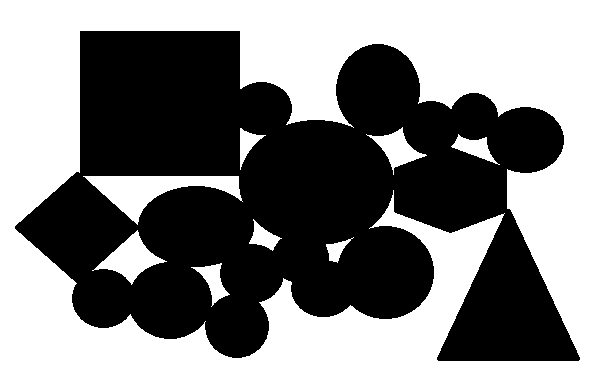
\includegraphics[scale=0.4]{bin.png}}
        \captionsetup{skip=0pt}
        \caption{Исходное изображение для задания 2}
        \label{fig:bin}
    \end{figure}
    Разделим наши фигуры морфологическими операциями. Далее будут приведены полученное изображение и оно же, но
    с выделенными краями. Так мы сможем увидеть, насколько хорошо фигуры отделились друг от друга.
    \begin{figure}[H]
        \centering
        \fbox{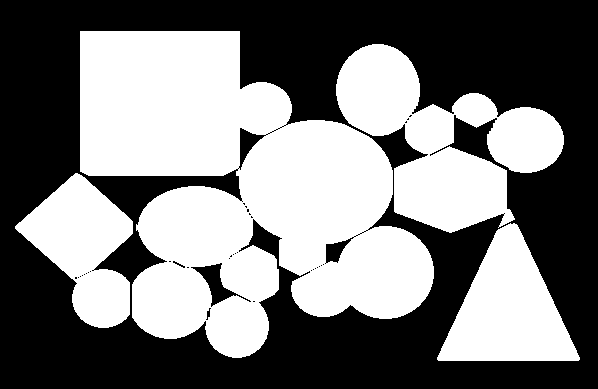
\includegraphics[scale=0.31]{bin_new.png}}
        \captionsetup{skip=0pt}
        \caption{Результат разделения фигур морфологическими операциями}
        \label{fig:binn}
    \end{figure}
    \begin{figure}[H]
        \centering
        \fbox{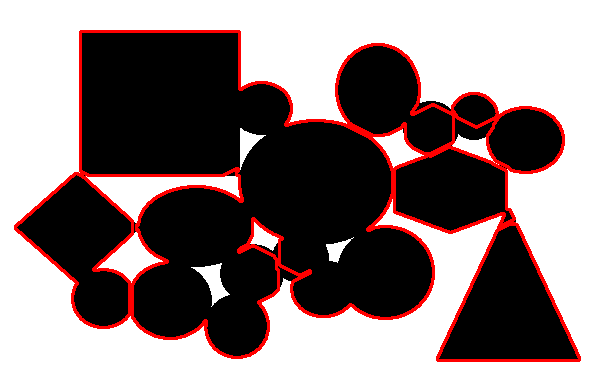
\includegraphics[scale=0.31]{bin_new_c.png}}
        \captionsetup{skip=0pt}
        \caption{Выделение контура}
        \label{fig:binnc}
    \end{figure}
    \begin{figure}[H]
        \centering
        \fbox{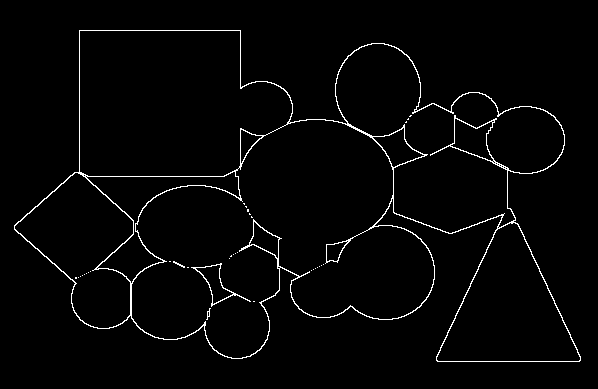
\includegraphics[scale=0.31]{bin_new_c2.png}}
        \captionsetup{skip=0pt}
        \caption{Выделение контура подходом $C=(A\oplus B)-A$}
        \label{fig:binnc2}
    \end{figure}
    Видим, что лучше всего разделяются окружности или овалы. Разделение <<склеенных>> объектов
    получилось неплохо, но некоторые фигуры деформировались или на них появились лишние линии
    разделения.


    \subsection{Листинг для задания 2}
    \begin{lstlisting}[label=task2, caption=Программа для разделения <<склеенных>> объектов]
    import cv2
    import numpy as np

    def separate_objs(I, iters, mellipse=(5,5)):
        ret, Inew = cv2.threshold(I, 160, 255, cv2.THRESH_BINARY_INV)
        B = cv2.getStructuringElement(cv2.MORPH_ELLIPSE, mellipse)

        BW2 = cv2.morphologyEx(Inew,
                            cv2.MORPH_ERODE,
                            B,
                            iterations=iters,
                            borderType=cv2.BORDER_CONSTANT,
                            borderValue=(0))

        T = np.zeros_like(Inew)
        while cv2.countNonZero(BW2) < BW2.size:
            D = cv2.dilate(BW2, B, borderType=cv2.BORDER_CONSTANT, borderValue=(0))
            C = cv2.morphologyEx(D,
                                cv2.MORPH_CLOSE,
                                B,
                                borderType=cv2.BORDER_CONSTANT,
                                borderValue=(0))
            S = C - D
            T = cv2.bitwise_or(S, T)
            BW2 = D

        T = cv2.morphologyEx(T,
                            cv2.MORPH_CLOSE,
                            B,
                            iterations=iters,
                            borderType=cv2.BORDER_CONSTANT,
                            borderValue=(255))

        Inew = cv2.bitwise_and(~T, Inew)
        return Inew

    def find_counters(Inew, col=(0, 0, 255), th=2):
        contours, _ = cv2.findContours(Inew, cv2.RETR_EXTERNAL,
                                       cv2.CHAIN_APPROX_SIMPLE)
        contour_I = cv2.cvtColor(Inew, cv2.COLOR_GRAY2BGR)
        cv2.drawContours(contour_I, contours, -1, col, th)
        return contour_I

    def outer_contour(A):
        B = cv2.getStructuringElement(cv2.MORPH_RECT, (3, 3))
        dilation = cv2.dilate(A, B)
        outer_contour = dilation - A
        return outer_contour

    if __name__ == '__main__':
        path = 'tv_lab6'
        src = 'source'
        render = 'renders'
        
        binary_I = cv2.imread(f"{path}/{src}/bin.png", cv2.IMREAD_GRAYSCALE)
    
        binary_Inew = separate_objs(binary_I, 10)
        c_im = find_counters(binary_Inew)
        c_im2 = inner_contour(binary_Inew)
        cv2.imwrite(f"{path}/{render}/bin_new.png", binary_Inew)
        cv2.imwrite(f"{path}/{render}/bin_new_c.png", c_im)
        cv2.imwrite(f"{path}/{render}/bin_new_c2.png", c_im2)
    \end{lstlisting}


    \section{Задание 3. Сегментация}
    В подходе сегментации по водоразделам изображение рассматривается как карта высот,
    на котором интенсивности пикселей описывают высоты относительно некоторого уровня.
    На такую <<высотную местность>> <<льет дождь>>, образуя множество водосборных бассейнов.
    Постепенно вода из переполненных бассейнов переливается, и бассейны объединяются в более крупные.
    Места объединения бассейнов отмечаются как линии водораздела. Если <<дождь>> остановить рано,
    тогда изображение будет сегментировано на мелкие области, а
    если поздно -- на крупные.
    
    
    В таком подходе все пиксели подразделяются на три типа:
    \begin{enumerate}
        \item локальные минимумы.
        \item находящиеся на склоне (с которых вода скатывается в один и тот же локальный минимум).
        \item локальные максимумы (с которых вода скатывается более чем в один минимум).
    \end{enumerate}
    При реализации данного метода необходимо определить водосборные бассены и линии
    водораздела путем обработки локальных областей и вычисления их характеристик.
    
    
    Алгоритм сегментации
    состоит из следующих шагов:
    \begin{enumerate}
        \item Вычисление функции сегментации. Как правило, для этого используется градиентное представление изображения.
        \item Вычисление маркеров переднего плана на основании связности пикселей каждого объекта.
        \item Вычисление маркеров фона, представляющих пиксели, не являющиеся объектами.
        \item Модифицирование функции сегментации с учетом взаиморасположения маркеров переднего плана и фона.
    \end{enumerate}
    В результате работы алгоритма будет получена маска, где пиксели одинаковых сегментов будут помечены одинаковыми метками
    и будут образовывать связную область.


    Выберем произвольное изображение, содержащее небольшое число локальных минимумов, после чего выполним сегментацию
    по водоразделам. Пусть это будет картинка бананов, взятая из интернета:
    \begin{figure}[H]
        \centering
        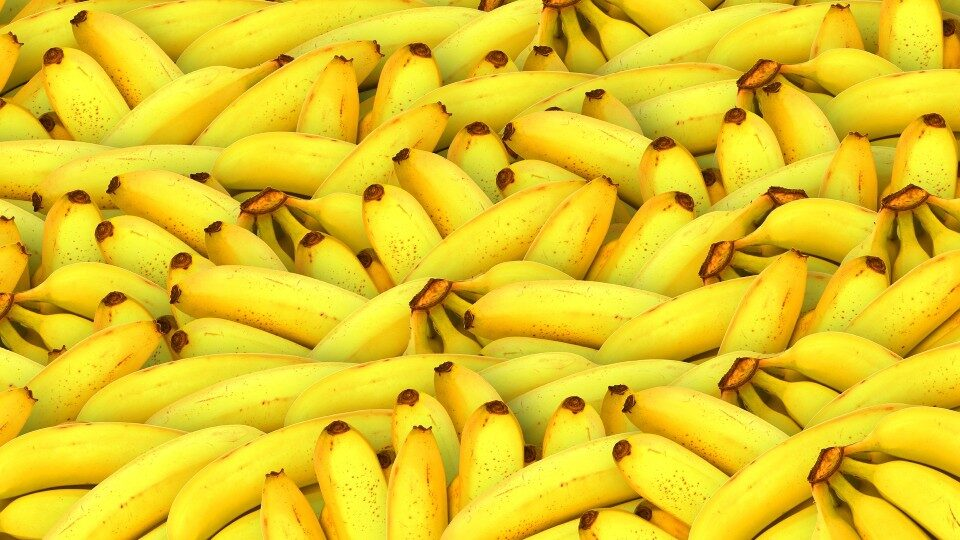
\includegraphics[scale=0.2]{seg.jpg}
        \captionsetup{skip=0pt}
        \caption{Исходное изображение для задания 3}
        \label{fig:seg}
    \end{figure}


    Применим сегментацию к изображению и получим следующее:
    \begin{figure}[H]
        \centering
        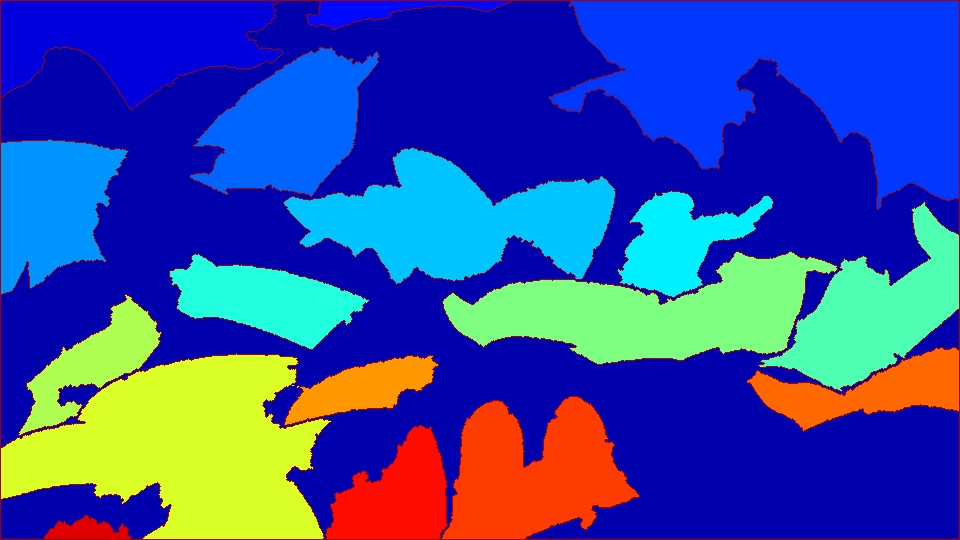
\includegraphics[scale=0.2]{seg_new_mj.jpg}
        \captionsetup{skip=0pt}
        \caption{Маркеры и границы, наложенные на изображение
        с использованием цветовой карты JET}
        \label{fig:segnj}
    \end{figure}
    \begin{figure}[H]
        \centering
        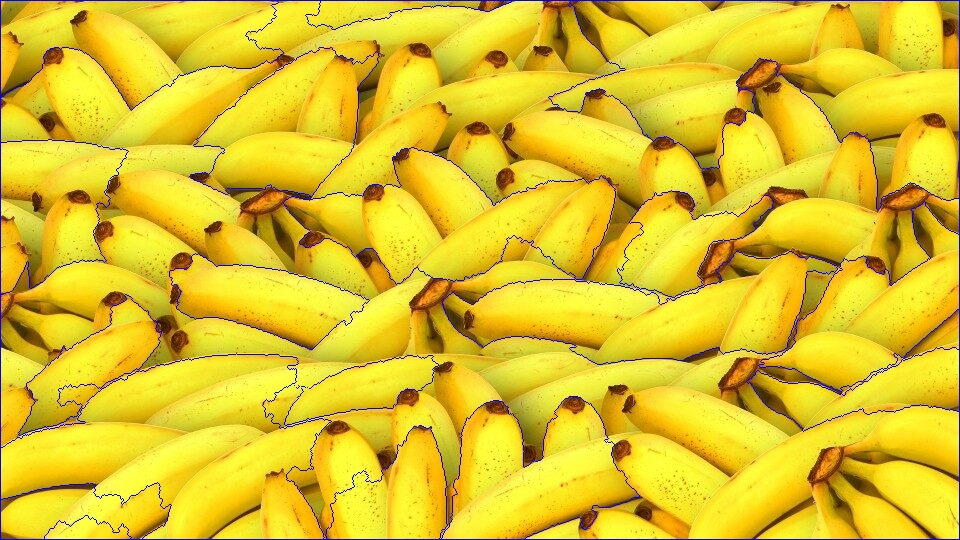
\includegraphics[scale=0.2]{seg_new.jpg}
        \captionsetup{skip=0pt}
        \caption{Сегментация исходного изображения (маркеры и границы, наложенные на исходное изображение)}
        \label{fig:segn}
    \end{figure}


    \subsection{Листинг для задания 3}
    \begin{lstlisting}[label=task3, caption={Программа для сегментации изображения}]
    import cv2
    import numpy as np

    def bwareaopen(A, dim, conn=8):
        if A.ndim > 2:
            return None

        num, labels, stats, centers = \
            cv2.connectedComponentsWithStats(A,
                connectivity = conn)

        for i in range(num):
            if stats[i, cv2.CC_STAT_AREA] < dim:
                A[labels == i] = 0
        return A


    def segmentation(I, dim, conn=8, mellpise=(5, 5), dis=5, coeff=0.6, color=(255, 0, 0)):
        I_gray = cv2.cvtColor(I, cv2.COLOR_BGR2GRAY)
        ret, I_bw = cv2.threshold(I_gray, 0, 255,
                                cv2.THRESH_BINARY + cv2.THRESH_OTSU)
        I_bw = bwareaopen(I_bw, dim, conn)
        B = cv2.getStructuringElement (\
            cv2.MORPH_ELLIPSE, mellpise)
        I_bw = cv2.morphologyEx (I_bw,\
                cv2.MORPH_CLOSE, B)

        I_fg = cv2.distanceTransform(I_bw, cv2.DIST_L2, dis)
        ret, I_fg = cv2.threshold(I_fg, coeff * I_fg.max(), 255, 0)
        I_fg = I_fg.astype(np.uint8)
        ret, markers = cv2.connectedComponents(I_fg)

        I_bg = np.zeros_like(I_bw)
        markers_bg = markers.copy()
        markers_bg = cv2.watershed(I, markers_bg)
        I_bg[markers_bg == -1] = 255

        I_unk = cv2.subtract(~I_bg, I_fg)

        markers = markers + 1
        markers[I_unk == 255] = 0

        markers = cv2.watershed(I, markers)
        markers_jet = cv2.applyColorMap(
            (markers.astype(np.float32) * 255 / (ret + 1)).astype(np.uint8),
            cv2.COLORMAP_JET)
        I[markers == -1] = color
        return I, markers_jet

    if __name__ == '__main__':
        seg_I = cv2.imread(f"{path}/{src}/seg.jpg", cv2.IMREAD_COLOR)
        
        seg_Inew, smj = segmentation(seg_I, dim=20, conn=4, mellpise=(5, 5), coeff=0.6)
        cv2.imwrite(f"{path}/{render}/seg_new.jpg", seg_Inew)
        cv2.imwrite(f"{path}/{render}/seg_new_mj.jpg", smj)
    \end{lstlisting}


    \section{Ответы на вопросы}
    \subsection{Включает ли результат открытия в себя результат закрытия?}


    \subsection{Какой морфологический фильтр необходимо применить, чтобы убрать у объекта выступы?}


    \subsection{Каким образом с помощью морфологических операций можно найти контур объекта?}


    \subsection{Что такое морфология?}


    \section{Вывод}
\end{document}